\chapter{Clustering Retweets}
\label{chap:cluster_retweets}
Wie in Abschnitt \ref{sec:struktur-eines-tweets} beschrieben enthält ein \gls{Retweet} die Informationen des/der Nutzer*in der/die ihn veröffentlicht hat, sowie die Informationen des/der Nutzer*in der/die den Original-Tweet veröffentlicht hat. Eine Beziehung kann hergestellt werden. Außerdem kann durch die Anzahl an \glspl{Retweet} der Beziehung eine Gewichtung zugeschrieben werden. Durch Analyse aller \glspl{Retweet} kann so ein Netz von Beziehungen zwischen Nutzern aufgebaut werden.
Werden in diesem Netz Nutzer*innen identifiziert, die sich häufig untereinander \glspl{retweetet} so können diese einer Gruppe zugeordnet werden. Im Folgenden soll der Prozess solche Gruppen zu finden dargestellt und die Ergebnisse präsentiert werden.

\section{Daten vorbereiten}
\label{sec:daten-vorbereiten}
Zur Verarbeitung und Analyse der Daten wurde keine Datenbank verwendet sondern ausschließlich mit Dateioperationen und Ordnerstrukturen gearbeitet. Somit können die Daten in jeder belieben Art und Strukturierung abgelegt, Metainformationen hinzugefügt und jeder Schritt des Prozesses kann zwischengespeichert werden. 
Um von Tweets auf Beziehung zwischen Nutzer*innen zu schließen wurden folgende Schritte ausgeführt:
\begin{enumerate}
	\item \textbf{Daten aus \gls{S3 - Bucket} herunterladen}
	\item \textbf{Unrelevante Informationen filtern}\\  So wird ein übersichtliches Format erreicht und Speicherplatz gespart. Das resuliertende Tweet-Objekt entspricht der Bespreibung aus Abschnitt \ref{sec:struktur-eines-tweets}
	\item \textbf{Tweets in einer Ordnerstruktur nach Nutzer sortieren\\} Als eindeutige Identifikation wurde der in Abschnitt \ref{sec:struktur-eines-tweets} genannte Nutzername gewählt. Es ensteht folgende Ordnerstruktur: \\
	\dirtree{%
		.1 /.
		.2 Nutzer1.
		.3 Tweet1.json.
		.3 Tweet2.json.
		.2 Nutzer2.
		.3 Tweet1.json.
		.3 Tweet2.json.
		.3 Tweet3.json.
	}

	\item \textbf{Metadaten erstellen}\\
	Nun soll für jede*n Nutzer*in Metadaten erstellt werden, von wem und wie oft er von anderen Nutzer*innen \gls{geretweetet} wurde.
	Dafür werden alle Nutzer*innen und ihre Tweets analysiert; ist einer davon ein \gls{Retweet} eines andere*n Nutzer*in so wird das, zusammen mit der Anzahl, in den Metdaten desjenigen Nutzers, der \gls{geretweetet} wurde, vermerkt. 
	Für jeden Nutzer entstehen damit Metadaten der Form:
	\lstset{
		string=[s]{"}{"},
		stringstyle=\color{blue},
		comment=[l]{:},
		commentstyle=\color{black},
	}
	
	\begin{lstlisting}[caption={Metdaten des Nutzer: "`tagesschau"'}]
		{
			"i_was_retweeted_by": {
				"RSplettsto": 2,
				"Roxana50189220": 2,
				"RobbyTipps": 14,
				"RafaelOsswald": 2,
				"rbbinforadio": 16
			},
			"i_am_retweeting": {
				"tagesthemen": 6,
				"ARD_BaB": 3,
				"aktuelle_stunde": 1,
				"gudrun_engel": 1
			}
		}
	\end{lstlisting}
\end{enumerate}
Dieser Prozess besitzt eine Komplexität von $\mathcal{O}(n)$ mit $n$ = Gesamtanzahl an Tweets. 
\section{Hauptfiguren identifizieren}
Bei der Untersuchung dieser Metadaten, ist aufgefallen, dass der Großteil aller \glspl{Retweet} auf einen kleinen Anteil aller Nutzer*innen fällt.
In Abbildung \ref{fig:tweetverteilung} ist diese Verteilung dargestellt; die Anzahl an \glspl{Retweet} nimmt annähernd expotentiell ab. 
\begin{figure}[h!]
	\centering
	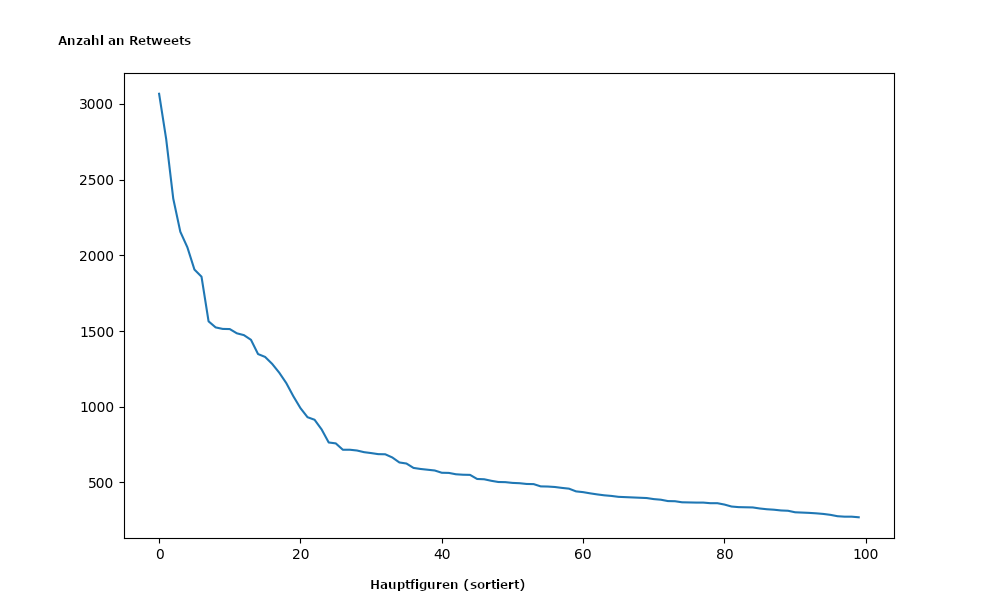
\includegraphics[width=0.8\linewidth]{images/Tweet_verteilung}
	\caption[]{Verteilung der Anzahl an \glspl{Retweet}}
	\label{fig:tweetverteilung}
\end{figure}
Daraus wurde der Schluss gezogen, dass Beziehungen zwischen "`kleineren"' Nutzer*innen vernachlässigbar sind und nur Verbindungen zu den z.B. 100 meist \glspl{geretweetet} Nutzer*innen von Bedeutung sind. Diese werden im Folgenden "`Hauptfiguren"' genannt. Auch kann davon ausgegangen werden, dass Beziehung zwischen "`kleineren Nutzern"'  repräsentiert sind, da zwei Nutzer*innen die sich gegenseitig \glspl{retweetet}, wahrscheinlich auch eine Beziehung zur gleichen Hauptfigur haben. 
Diese Methodik vermindert die Anzahl an Verbindungen und führt zu einer effizenteren Verarbeitung der Daten sowie später zu einem übersichtlicheren Graphen (siehe Abschnitt %%%%%)
Die Anzahl an Hauptfiguren ist wählbar führt zu verschiedenen Ergebnisse, allerdings hat sich 100 als ein passender Parameter herausgestellt. Dieser Sachverhalt wird in Abschnitt näher diskutiert.

\section{Nutzergruppen aggregieren}
 Hauptfiguren $H$ und Nutzer*innen $N$ können als Knoten $K = H \cup N$,  Beziehungen als gewichtete Kanten $E$ eines Graphen $G = (K,E)$ betrachtet werden.
Dieser kann als ungerichtet definiert werden, da Kanten immer zu einer Hauptfiguren zeigen.
$E$ ist hierbei eine Menge an Paaren der Form ($h\in H$,$n\in  N$,$g$) wobei $g$ die Anzahl der \gls{Retweet} darstellt. 
Dieser Graph kann visualisiert werden. Genutzt wurde dafür \gls{Python3}, \gls{Matplotlib} und eine NEATO Implementierung als \gls{Layoutalgorithmus} (siehe \footfullcite{neato}).
\begin{figure}[h]
	\centering
	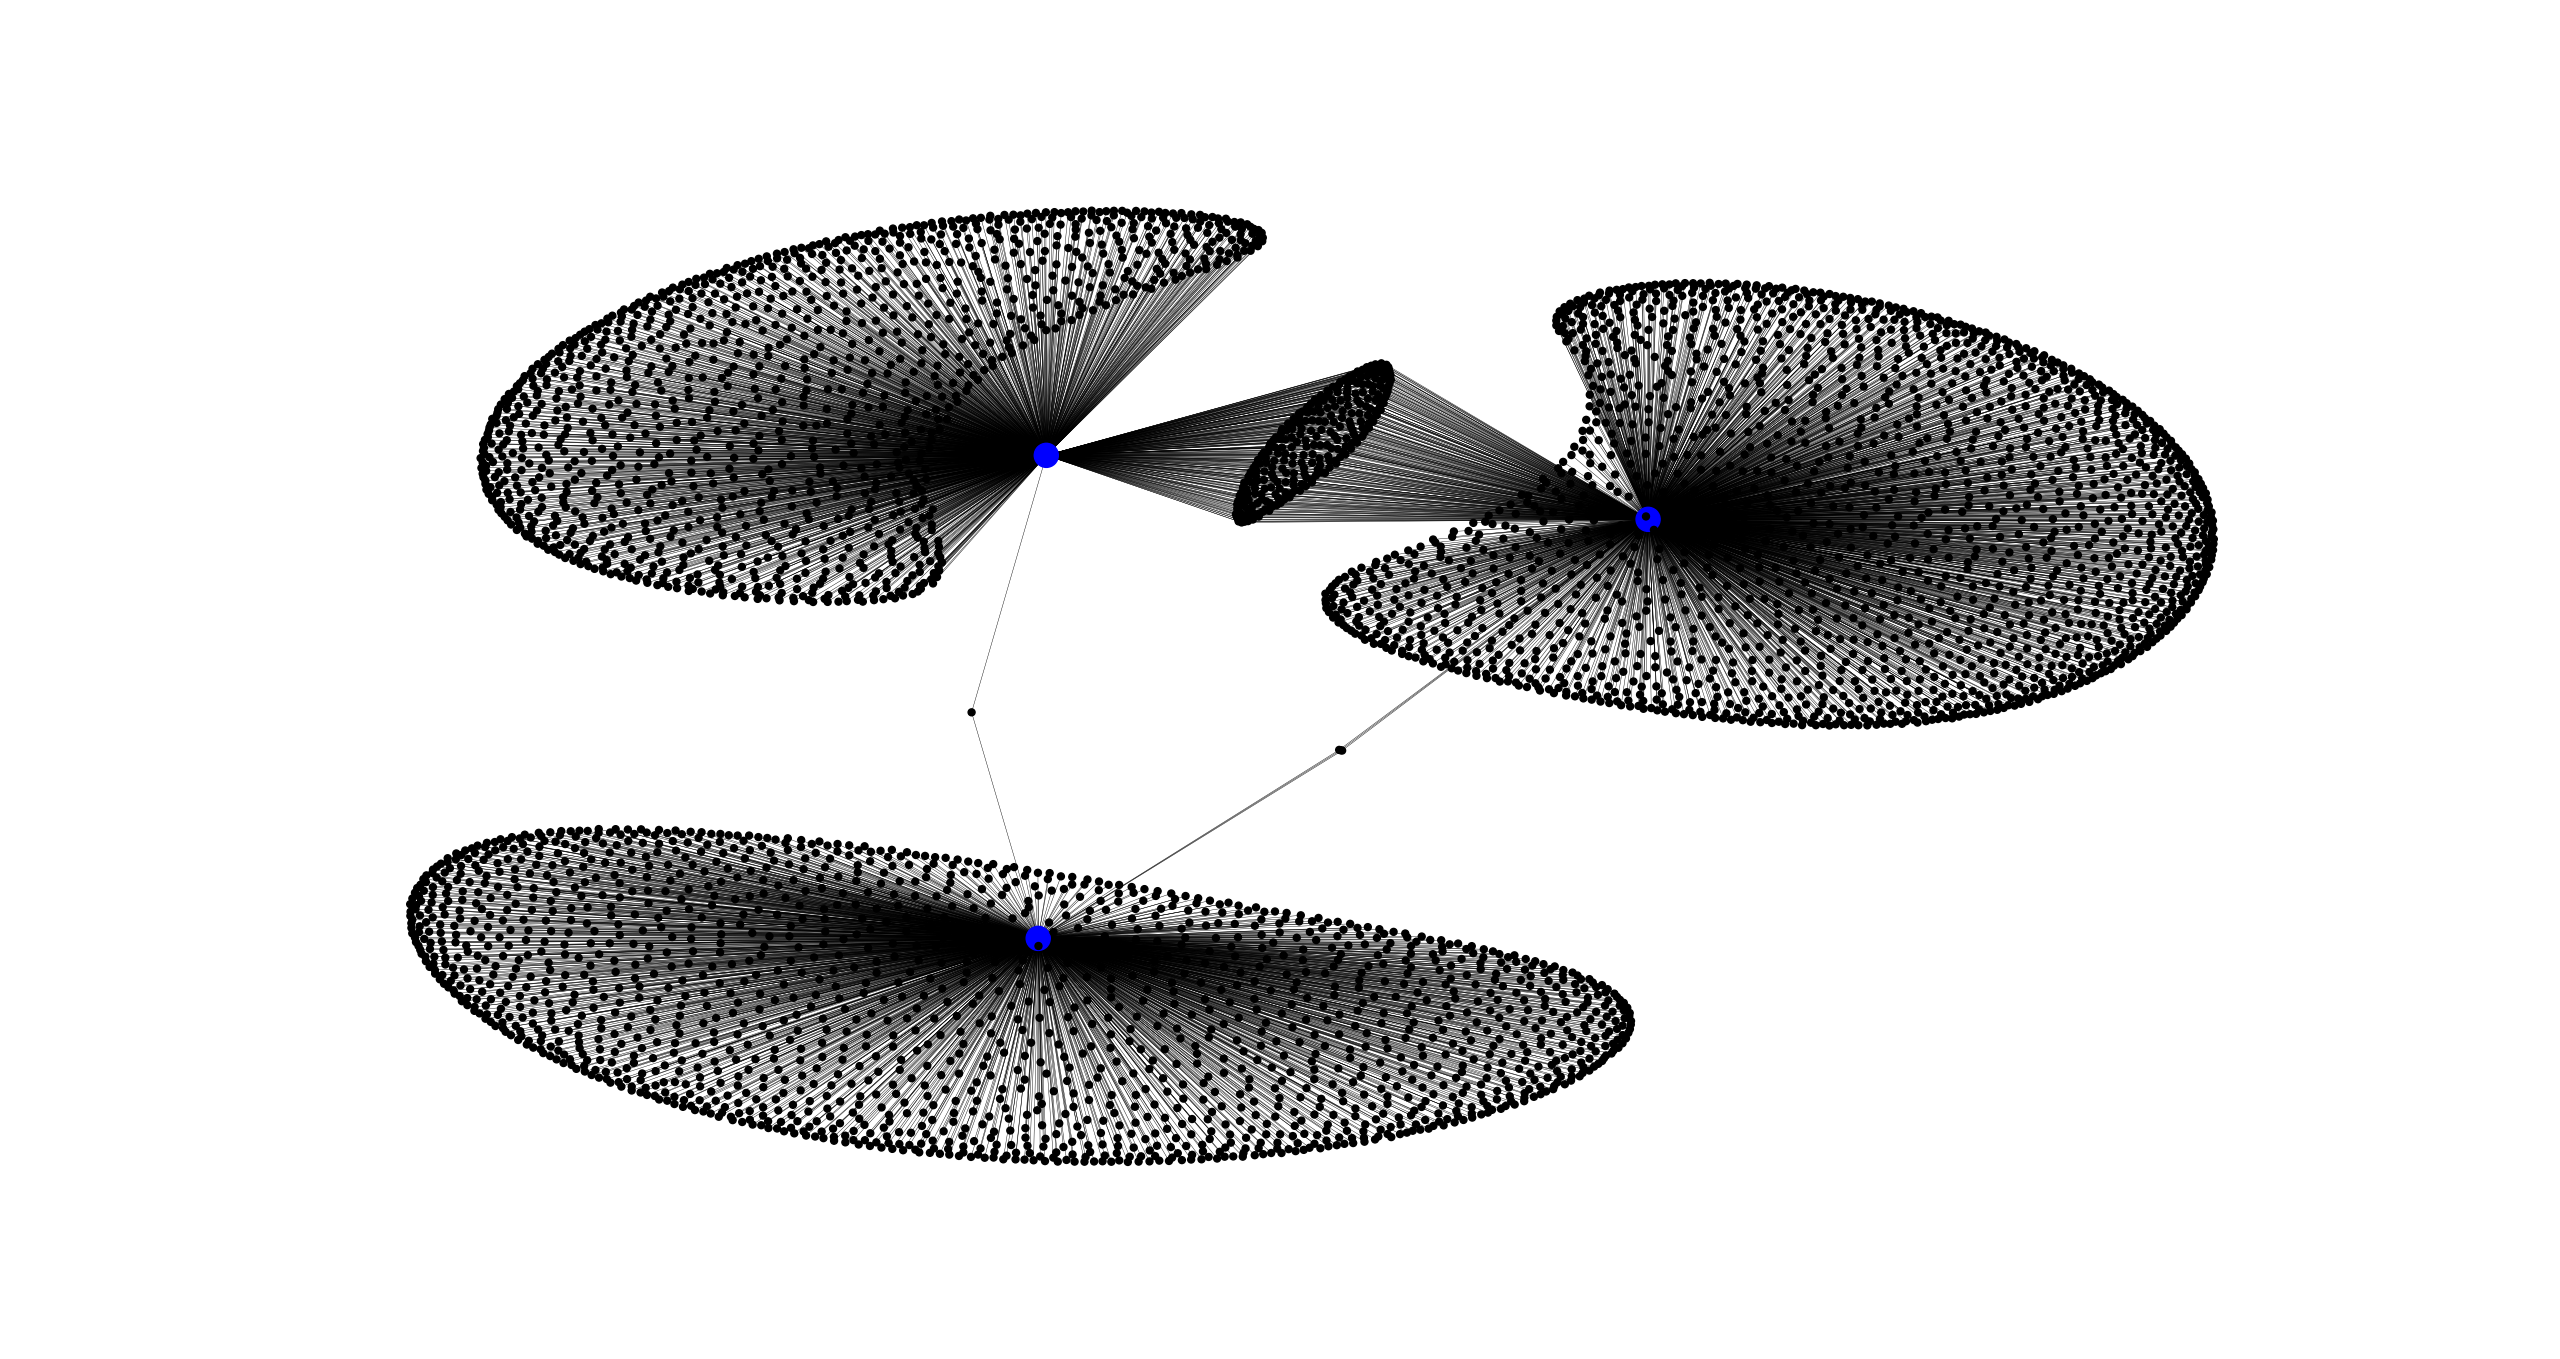
\includegraphics[width=\linewidth]{images/GraphNoAggregation}
	\caption[]{Graph mit drei Hauptfiguren (blau)}
	\label{fig:graphnoaggregation}
\end{figure}

Abbildung \ref{fig:graphnoaggregation} zeigt einen solchen Graph mit Daten aus 4 Tagen, den drei Hauptfiguren in blau (Karl\_Lauterbach, reitschuster, Volksverpetzer) und allen Nutzer*innen die diese \gls{geretweetet} haben in schwarz. Die Berechnung dieses Layout braucht auf einen handelsüblichen PC mit Linux 35,6 Sekunden. 
Mit Daten von mehr als 4 Tagen oder mit mehr als 3 Hauptfiguren explodiert die Berechnungszeit. 
Offensichtlich erkennbar ist, dass es  für jede Hauptfigur eine Menge an Nutzer*innen $N_{h^x}$ gibt, die nur diese Hauptfigur \gls{geretweetet} haben.
Analog dazu gibt es eine Menge an Nutzer*innen $N_{h^1h^2}$ die sowohl Hauptfigur $h^1$ und Hauptfigur $h^2$. 
Diese Mengen können als "`Superknoten"' betrachtet werden, der alle Nutzer*innen repräsentiert, die z.B. sowohl $h^1$ als auch $h^2$ \gls{geretweetet} haben.
Es gilt also für einen Superknoten$s$:
 \begin{equation}
s_{h^n\,..\,h^m} = \{n\in N|\exists e(n,h^n\,..\,h^m)\in E\}
\end{equation}
Die Gewichte $g$ der Kanten werden aufaddiert. 
Damit lässt sich der Graph auf maximal
\begin{equation}
|K| = |S| + |H| = \sum_{n=1}^{|H|} \binom{|H|}{n} + |H|
\end{equation}
Knoten beschränken (mit $S$ der Menge aller möglichen Superknoten).
\begin{figure}[h]
	\centering
	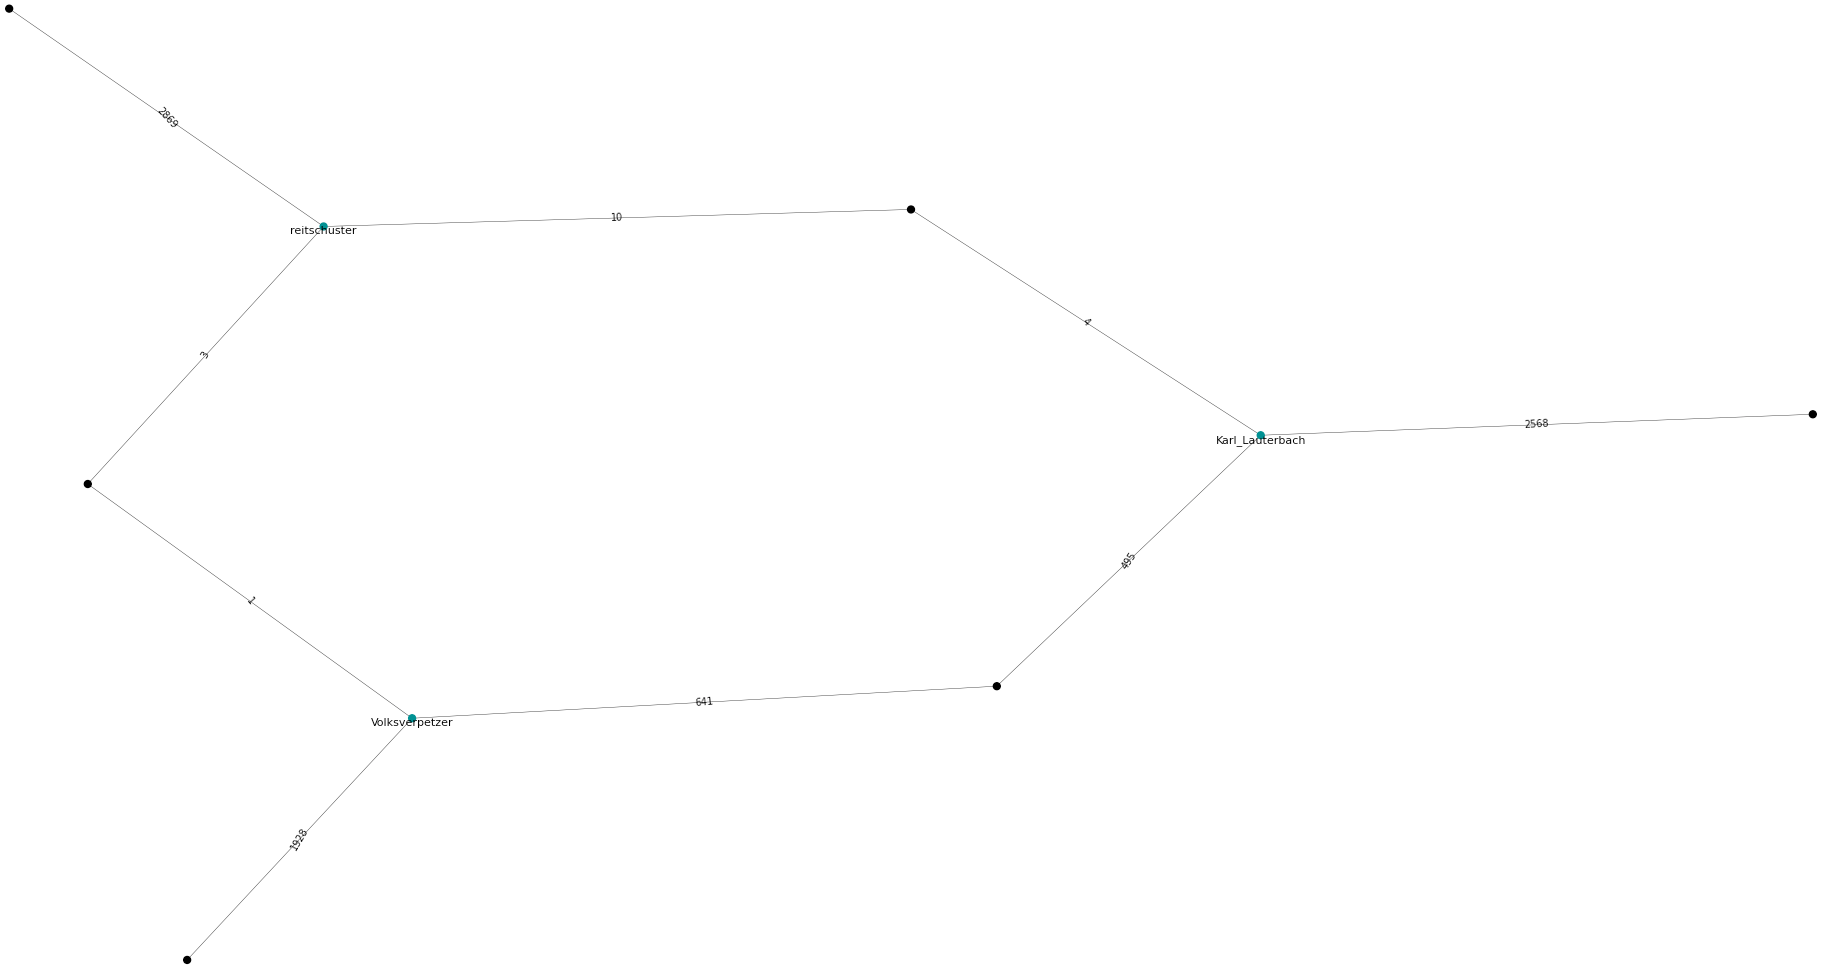
\includegraphics[width=0.7\linewidth]{images/GraphNoThreshold}
	\caption{Graph mit aggregierten Superknoten}
	\label{fig:graphnothreshold}
\end{figure}
Abbildung \ref{fig:graphnothreshold} zeigt den selben Graph wie \ref{fig:graphnoaggregation} mit zu Superknoten aggregierten Nutzern.
Die Berechnung des Layout konnte dadurch auf 0.16 Sekunden reduziert werden.
Auch dieser Prozess besitzt eine Komplexität von $\mathcal{O}(n)$ mit $n$ = Gesamtanzahl an Nutzern. 
\section{Kanten filtern}
Wie in Abbildung \ref{fig:superknotenentwicklung} zu sehen, steigt die Anzahl an möglichen Superknoten sehr schnell mit steigender Zahl an Hauptfiguren.
\begin{figure}[h]
	\centering
	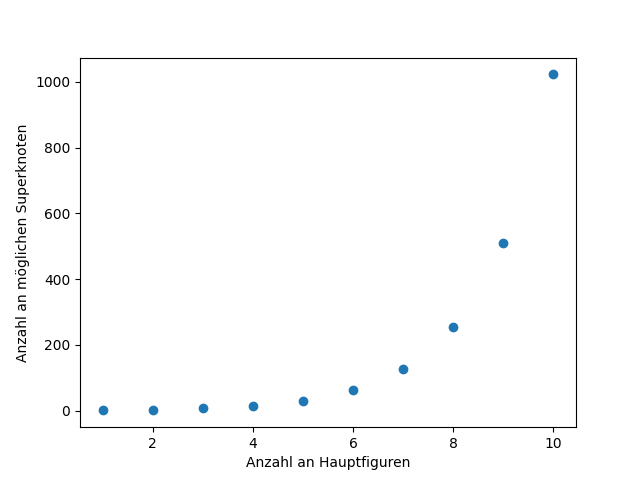
\includegraphics[width=0.7\linewidth]{images/Superknotenentwicklung}
	\caption[]{Entwicklung der möglichen Superknoten mit der Anzahl an Hauptfiguren}
	\label{fig:superknotenentwicklung}
\end{figure}
Bei $|H| = 100$ könnten bis zu $1.26*10^{30}$ Superknoten existieren. Das ist für jegliche Berechnung oder Darstellung unpraktikabel.
Deshalb wird auch hier eine Komplexitätsverringerung durch Filtern unrelevanter Information vorgenommen indem alle Kanten von einem Superknoten zu einer Hauptfigur gelöscht werden, die unter einem Schwellwert liegen. 
Es wird davon ausgegangen, dass  bei einem niedrigen Kantengewicht die Nutzer*innen nur eine schwache Beziehung zu dem entsprechenden Hauptakteur haben und diese damit für eine spätere Gruppierung irrelavant ist. 
Wie dieser Schwellenwert festgelegt wird, wird in Abschnitt diskutiert. 
Es gilt also mit dem Schwellwert $T$: \begin{equation}
	E_{gefiltert} = \{(s,h,g)\in E|g>T\}
\end{equation}

Wurde eine Kante (z.B. $(s,h3)$) von einem Superknoten $s_{h^1h^2h^3}$ gelöscht, so ändert sich dieser zu $s_{h^1h^2}$. Nun ist es allerdings möglich, dass der Knoten $s_{h^1h^2}$ bereits existiert, was zu einer Verdopplung der eigentlich gleichen Kante führt. Dies kann vermieden werden indem nach dem Löschen einer Kante überprüft wird ob der so enstandene Superknoten bereits existiert. Falls ja, werden diese zusammengeführt indem die jeweiligen Kantengewichte addiert werden.
Des Weiteren werden diejenigen Superknoten geschlöscht, die Nutzer repräsentierten, die nur eine Hauptfigur \gls{geretweetet} haben, da sie für eine Eingruppierung anhand von Beziehung keine Relevanz haben.
Dieser Prozess besitzt eine Komplexität von $\mathcal{O}(n^2)$ mit $n$ = Gesamtanzahl der Superknoten, da im schlechtesten Fall für jeden veränderten Knoten, dieser mit alle bereits bestehenden Knoten auf Gleichheit überprüft werden muss.
\section{Clustering}
Das Ergebnis aller bisherigen Prozessschritte mit den Daten von März 2021 (ca. 2,5 Millionen Tweets, 260.000 Nutzer), 100 Hauptfiguren und einem Schwellenwert von 61 ist in Abbildung \ref{fig:noclusters} zu sehen und wurde innerhalb von 2 Stunden und 58 Minuten berechnet. 
\begin{figure}[h!]
	\centering
	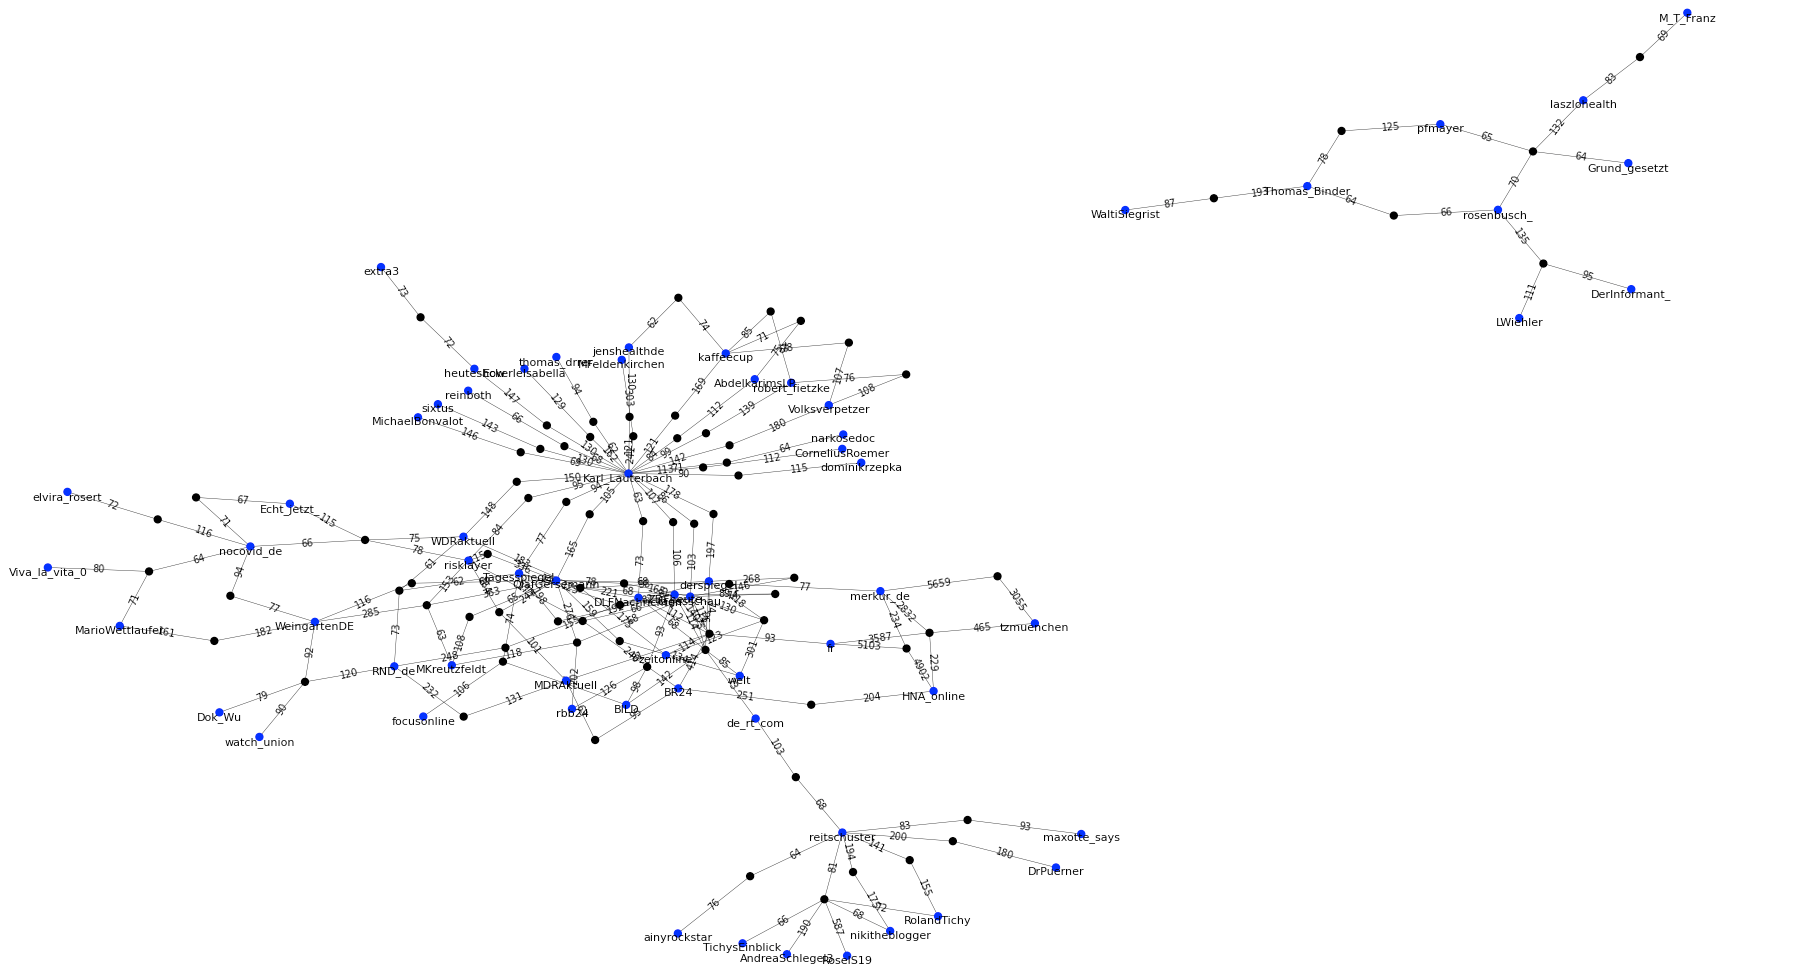
\includegraphics[width=\linewidth]{images/NoClusters}
	\caption[]{Ergebnisgraph März 2021}
	\label{fig:noclusters}
\end{figure}









